\section{Installation}

The repository at  \url{https://github.com/datafl4sh/shimmer.git}  includes shimmer++ library sources, the original matlab code from where it is based (not a direct translation). In addition, there is a bunch of documents that along with the github issues record the developments of shimmer++.  
\subsection{Get your local copy of the repository}
Before cloning the repository, its a good practice to first update your system. For Debian-based operational system: 
    \begin{verbatim}
        sudo apt update
    \end{verbatim}    
You should proceed by installing dependencies. The main additional libraries are Eigen and Boost Graph Library (BGL). The first is concerned with the linear algebra while the latter with the graph representation. As usual,  we use cmake/make/g++ to built/compile/run the project and git for tracking purposes.  \cred{Maybe add sthg about C++>17, gcc, clang}
For Debian-based operational system: 
\begin{verbatim}
    sudo apt install -y  make cmake build-essential git ctest; 
    sudo apt install -y  libeigen3-dev;
    sudo apt install -y  libboost-graph-dev libboost-dev
\end{verbatim}
To download the sources see:
\begin{itemize}
    \item For BGL \url{https://sourceforge.net/projects/boost/}
\end{itemize}

Use the following link \url{https://eigen.tuxfamily.org/dox/AsciiQuickReference.txt} for a quick comparison of Eigen and Matlab.

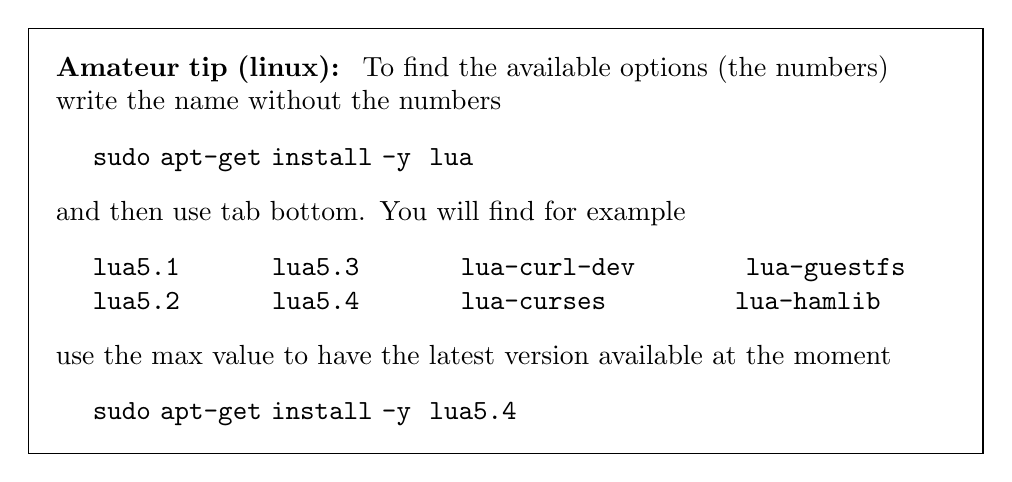
\begin{tikzpicture}
\node [draw,text width=\linewidth-20pt, inner sep=10 pt]%
{
\textbf{Amateur tip (linux):}                                                                   \      
To find the available options (the numbers) write the name without the numbers                  
\begin{verbatim}
    sudo apt-get install -y  lua   
\end{verbatim}
and then use tab bottom. You will find for example                       
\begin{verbatim}
    lua5.1          lua5.3           lua-curl-dev            lua-guestfs        
    lua5.2          lua5.4           lua-curses              lua-hamlib          
\end{verbatim}
use the max value to have the latest version available at the moment                   
\begin{verbatim}
    sudo apt-get install -y  lua5.4
\end{verbatim}
};
\end{tikzpicture}    
Now you are ready to clone the repository using one the following alternatives lines
\begin{verbatim}
    git clone git@github.com:datafl4sh/shimmer.git        
    git clone https://github.com/datafl4sh/shimmer.git
\end{verbatim}

\subsection{Building shimmer++}
To build shimmer++ use the standard ccmake/make steps knowing that the CMakeList.txt is in the shimmer++ directory.
\begin{verbatim}
    ccmake "path_to_shimmer++_directory"         
    make  
\end{verbatim}


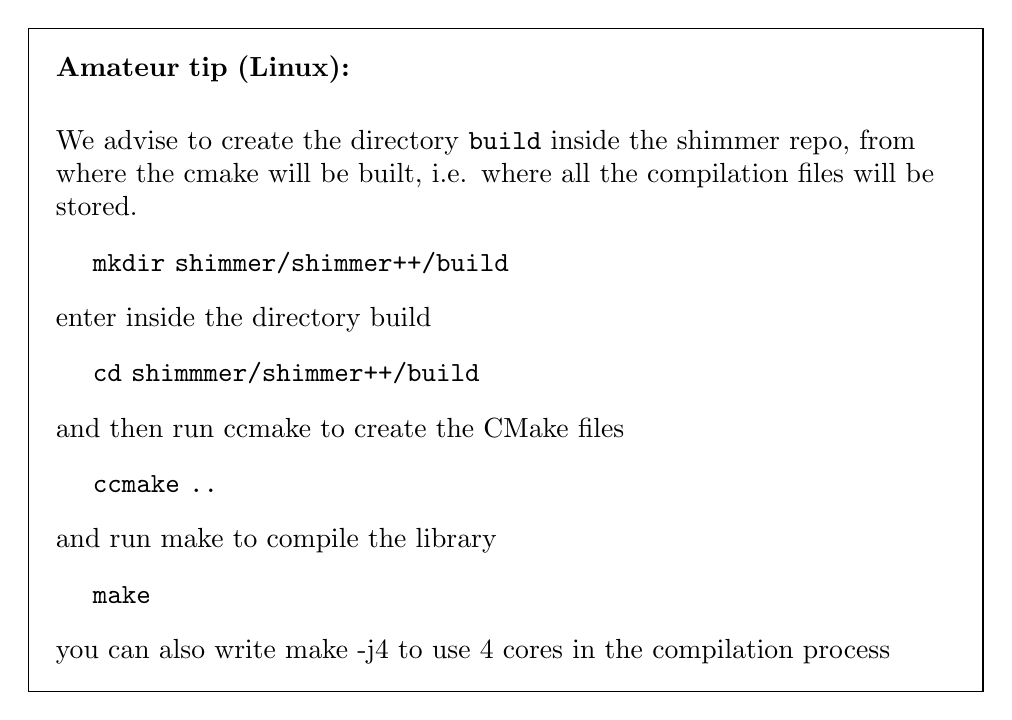
\begin{tikzpicture}
    \node [draw,text width=\linewidth-20pt, inner sep=10 pt]%
{
\textbf{Amateur tip (Linux):}
\vspace{5mm} \\
We advise to create the directory \texttt{build} inside the shimmer repo, from where  the cmake will be built, i.e. where all the compilation files will be stored. 
\begin{verbatim}
    mkdir shimmer/shimmer++/build
\end{verbatim}
enter inside the directory build
\begin{verbatim}
    cd shimmmer/shimmer++/build
\end{verbatim}
and then run ccmake to create the CMake files
\begin{verbatim}
    ccmake ..
\end{verbatim}
and run make to compile the library
\begin{verbatim}
    make
\end{verbatim}
you can also write make -j4 to use 4 cores in the compilation process};
\end{tikzpicture}

\subsection{Shimmer++ organization}
The library is mainly organised with sources stored in the \texttt{shimmer/shimmer++/src} folder and unitary tests in the \texttt{shimmer/shimmer++/unit\_tests}. There is an additionally GERG folder which accounts for the interface of shimmer++ with the code regarding GERG computations.

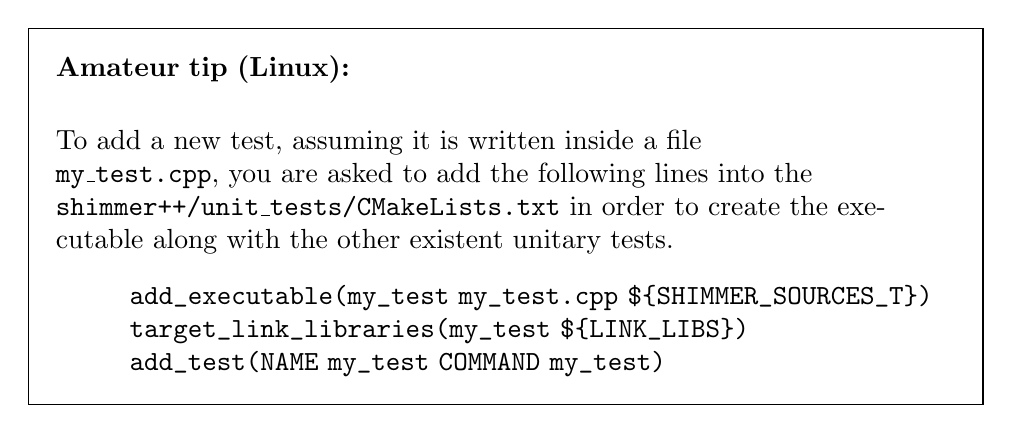
\begin{tikzpicture}
    \node [draw,text width=\linewidth-20pt, inner sep=10 pt]
{
\textbf{Amateur tip (Linux):}
\vspace{5mm} \\
To add a new test, assuming it is written inside a file \texttt{my\_test.cpp}, you are asked to add the following lines into the \texttt{shimmer++/unit\_tests/CMakeLists.txt} in order to create the executable along with the other existent unitary tests.
\begin{verbatim}
        add_executable(my_test my_test.cpp ${SHIMMER_SOURCES_T})
        target_link_libraries(my_test ${LINK_LIBS})
        add_test(NAME my_test COMMAND my_test)
\end{verbatim}
};
\end{tikzpicture}


